\documentclass[tikz,border=8pt]{standalone}
\begin{document}
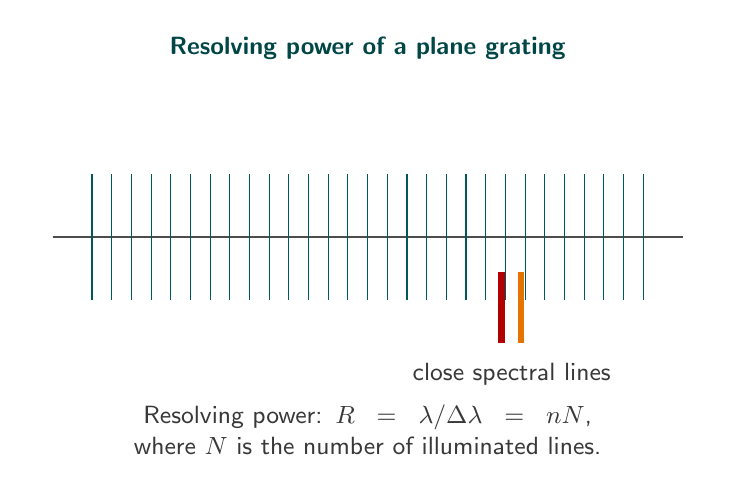
\begin{tikzpicture}[
  line/.style={draw=black!70,line width=0.75pt},
  label/.style={font=\sffamily\small,text=black!78},
  title/.style={font=\sffamily\bfseries\small,text=teal!55!black},
]
\node[title] at (0,2.4) {Resolving power of a plane grating};
\draw[line] (-4,0)--(4,0);
\foreach \x in {-3.5,-3.25,...,3.5}{\draw[teal!70!black] (\x,-0.8)--(\x,0.8);}
\draw[red!70!black,line width=2.2pt] (1.7,-1.35)--(1.7,-0.45);
\draw[orange!90!black,line width=2.2pt] (1.95,-1.35)--(1.95,-0.45);
\node[label] at (1.83,-1.75) {close spectral lines};
\node[label,align=center,text width=8.4cm] at (0,-2.45)
  {Resolving power: $R=\lambda/\Delta\lambda=nN$, where $N$ is the number of illuminated lines.};
\end{tikzpicture}
\end{document}
